\documentclass[11pt]{article}

\usepackage{sectsty}
\usepackage{graphicx}
\usepackage[T1]{fontenc}
\usepackage{epigraph} %quotes
\usepackage{amssymb} %math symbols
\usepackage{mathtools} %more math stuff
\usepackage{amsthm} %theorems, proofs and lemmas
\usepackage[ruled,vlined]{algorithm2e} %algoritms/pseudocode
\usepackage{bm}

\newcounter{thecnt}[section]
\def\thecnt{\arabic{}}

%% Theorem notation
\newtheorem{theorem}{Theorem}
\newtheorem{corollary}{Corollary}
\newtheorem{claim}{Claim}
\newtheorem{lemma}{Lemma}
\newtheorem{problem}{Problem}
\newtheorem{definition}{Definition}
\newtheorem{remark}{Remark}

%% declaring abs so that it works nicely
\DeclarePairedDelimiter\abs{\lvert}{\rvert}%
\DeclarePairedDelimiter\norm{\lVert}{\rVert}%

% Swap the definition of \abs* and \norm*, so that \abs
% and \norm resizes the size of the brackets, and the 
% starred version does not.
\makeatletter
\let\oldabs\abs
\def\abs{\@ifstar{\oldabs}{\oldabs*}}
%
\let\oldnorm\norm
\def\norm{\@ifstar{\oldnorm}{\oldnorm*}}
\makeatother

% Marges
\topmargin=-0.45in
\evensidemargin=0in
\oddsidemargin=0in
\textwidth=5.5in
\textheight=9.0in
\headsep=0.5in


\title{Homework Set 2 - Networks out of Control}
\date{\today}
\author{Titouan Renard}

\begin{document}
\maketitle	

\section*{Exercise 1}


\begin{claim}
    Given that $n$ is even, using Stirling's formula, we claim that:
    \[ (n-1)!! \approx \alpha n^{n/2}e^{-n/2}, \]
    for some $\alpha \in \mathbb{R},~\alpha>0$ to be determined.
\end{claim}

\begin{proof}
    Recall that the double factorial of a number $n \in \mathbb{Z}$, denoted $n!!$, is given by the expression: 
    \begin{align*}
        n!! = \prod_{k=0}^{\frac{n}{2}} (n-2k) = n \cdot (n-2)  \cdot ... 3 \cdot 1 && \text{for an odd number,} \\
        n!! = \prod_{k=0}^{\frac{n+1}{2}} (n-2k) = n \cdot (n-2)  \cdot ... 4 \cdot 2 && \text{for an even number.} 
    \end{align*}
    Since $n$ is even we have that $n-1$ is odd. Observe that the expression
    \[ (n-1)!! = (n-1) \cdot (n-3)  \cdot ... 3 \cdot 1 \]
    can be expressed as (let $n=2k$, by $n$ even $k\in\mathbb{Z}$): 
    \begin{align*}
        (n-1)!! = \frac{(n-1) \cdot (n-2) \cdot (n-3) \cdot ... 3 \cdot 2 \cdot 1}{(n-2) \cdot (n-4) \cdot ... 4 \cdot 2} \\
        = \frac{(2k-1) \cdot (2k-2) \cdot (2k-3) \cdot ... 3 \cdot 2 \cdot 1}{(2k-2) \cdot (2k-4) \cdot ... 4 \cdot 2} = \frac{(2k-1)!}{2^{k-1}(k-1)!}.
    \end{align*}
    Which we reduce into:
    \begin{align*}
        (n-1)!! =  \frac{(2k-1)!}{2^{k-1}(k-1)!} = \frac{\frac{1}{n}*(n)!}{2^{k-1}(n/2)!*\frac{2}{n}} = \frac{1}{2^k} \frac{(n)!}{(n/2)!},
    \end{align*}
    by Stirling's formula we further get:
    \begin{align*}
        \frac{(n)!}{2^{n/2}(n/2)!} \approx  \frac{n^{n} e^{-n} \sqrt{2 \pi n}}{2^{n/2}((\frac{n}{2})^{n/2} e^{-n/2} \sqrt{\pi n})} = \sqrt{2}n^{n/2}e^{-n/2},
    \end{align*}
    where $\sqrt{2} = \alpha$.
\end{proof}

\newpage

\section*{Exercise 2} 

\begin{definition}
    A graph $G=(V,E)$ is said to be $k$-connected if there are at least $k$ vertex disjoint path between any two vertices $u,v\in V$ in $G$.
\end{definition}

\begin{theorem}
    (Connectivity of $G(n,r)$). For $r\geq 3$. $G(,r)$ is $r$-connected a.a.s. .
\end{theorem}

\begin{definition}
    Partition the vertex set $V$ of the graph the graph $G=(V,E)$ into 3 $A,B,S$ disjoint partitions s.t. $A\cup S \cup B=V$. We say that the set $S\subset V$ \textbf{separates} $G$ if $\not \exists ~ (u,v) \in E$ s.t. $u\in A,~v\in B$. 
\end{definition}

\begin{remark}
    If a graph $G=(V,E)$ is $k$ connected $\iff$ the size of the smallest set $S$ that separates $A$ and $B$ is $k$.
\end{remark}

\begin{proof} (of theorem 1)
    We separate the proof into two subcases, pick an arbitrary large number $a_0 \in \mathbb{Z}^+$, we distinguish the proof between two components, the \textbf{small component case} for $a=|A|<a_0$ and the \textbf{large component case} $a=|A|>a_0$.
    \linebreak

    For the \textbf{small component case} the proof is included in the lecture notes.
    \linebreak
    For the \textbf{large component case} we use a proof similar to the case $2<a<a_0$ from the small component proof.
    \begin{center}
        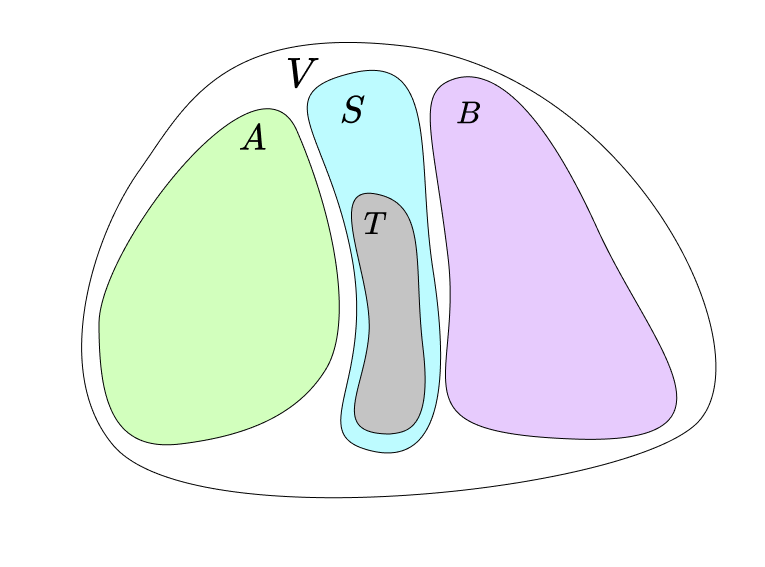
\includegraphics[width=0.4\textwidth]{figures/1.png}
    \end{center}
    Partition $V$ into three disjoint subsets $A,~B,~S$ s.t. $A\cup B\cup S=V$ and $S$ separates $A$ and $B$. Let $T\subseteq S$ be the subset of vertices in $S$ adjacent to $A$, let $t=|T|$ and $s=|S|$ and $a=|A|$. To show our result, we lower-bound $t$ and therefore $s$, by \textit{remark 1}, this is equivalent to showing that $G$ is $r$-connected. Let $H$ be the subgraph of $G$ that spans $T \cup A$. As in the small component proof, we have that $v(H) = a + t$ and $e(H) \geq \frac{ra + t}{2}$. To show that $G$ is $r$-connected we proceed by contradiction. We use the result from \textit{theorem 4.2 from the lecture notes} that states that a subgraph $H$ has a number of copies $\theta(n^{v(H)-e(H)})$. We will show that if $r>t$, then we can choose $a_0$ s.t. the number of copies of $H$ is $O(n^{-2})$, which will allow us to prove the $r$-connected claim. Suppose that $r>t$, then we have that:

    \begin{align*}
        e(H)-v(H) \leq (a+t) - \frac{ra + t}{2} 
    \end{align*}

    We want to show that $e(H)-v(H) \leq -2$, so with a bit of algebra we have: 

    \begin{align*}
        (a+t) - \frac{ra + t}{2}  \leq -2\\
        2a+2t - ra + t  \leq -4\\
        a(2-r) + t  \leq -4\\
        a  \geq \frac{\overbrace{-4-t}^{<0}}{\underbrace{2-r}_{<0}}.
    \end{align*}

    So letting $a_0 >  \frac{{-4-t}}{{2-r}}$ gives us that \# of occurrences of $H$ is $O(n^{-2})$. From that we get that:

    \begin{align*}
        \mathbb{P}\left[\text{$\exists$ the smallest $S$ has $|S|<r$ for any $n$}\right] = \\
        \sum_{a_0}^n  \mathbb{P} \left[\text{$\exists$ the smallest $S$ has $|S|<r$ for some $n$}\right] \\
        \leq n \cdot O(n^{-2}) = O(n^{-1}) \rightarrow 0,
    \end{align*}
    which completes the proof.
\end{proof}

\newpage

\section*{Exercise 3}

\subsection*{Question 1.} 
Let $X$ be generated from the $G(n,p)$ model and $Y$ be generated from the $G(n,r)$ model, i.e. sampled uniformly from the set pf $r$-regular graphs $\mathcal{G}(n,r)$ graphs. If $G$ is a $r$-regular is $\mathbb{P}\left[X=G|\text{$X$ is $r$-regular}\right]$ the same as  $\mathbb{P}\left[Y=G\right]$ ?
\BlankLine

Let $\bm{G_{r,n}}$ be the set of all possible $r$-regular graphs on $n$ vertices, observe that sampling from $G(n,p)$ and restricting to $r$-regular graphs or sampling $G(n,r)$ has in both case the effect of uniformly sampling through $\bm{G_{r,n}}$. Observe that:

\[ \mathbb{P}\left[X=G|\text{$X$ is $r$-regular}\right] = \mathbb{P}\left[Y=G\right] = \frac{1}{|\bm{G_{r,n}}|}. \] 

The probability doesn't depend on the sampling method.

\subsection*{Question 2.} 

We use the $G^*(n,r)$ matching construction to prove r-regular graph properties instead of the Erdòs-Rény model since properties that hold from $G^*(n,r)$ hold a.a.s for $G(n,r)$, which is not true of the $G(n,p)$ model.
% We do not use this model to prove properties on $X$ because the Erdòs-Rény model and its properties are useless to

\end{document}